\documentclass[11pt,a4paper,oneside, reqno]{amsproc}
\usepackage{changepage}
\usepackage{mathtext} % русские буквы в формулах
\usepackage[T2A]{fontenc}
\usepackage[utf8x]{inputenc}
\usepackage{ucs}
\usepackage{cmap}
\usepackage[english,russian]{babel}
\usepackage{graphicx}
%\usepackage{concrete}
%\usepackage{amsmath}
%\usepackage{amsfonts}
\usepackage{amssymb}
\usepackage{dcolumn}
\usepackage{booktabs}
\usepackage{ctable}
\usepackage{multirow}

\newcommand{\specialcell}[2][c]{%
  \begin{tabular}[#1]{@{}c@{}}#2\end{tabular}}
\oddsidemargin = 0pt
\textwidth = 14 cm
\topmargin = -2 cm
\textheight = 24 cm
\makeatletter
\renewcommand{\theequation}{\thesection.\arabic{equation}}
\@addtoreset{equation}{section}
\newcommand{\eq}{\begin{equation}}
\newcommand{\eeq}{\end{equation}}
\newcommand{\fr}{\frac}
\newcommand{\mf}{\mathfrak}
\newcommand{\sub}{\subsection}
\newcommand{\subsub}{\subsubsection}
\newcommand{\definition}{\theoremstyle{definition}}
\newcommand{\mult}[2]{\genfrac{\left[}{\right.}{0pt}{}{#1}{#2}}
\renewcommand{\qed}{\begin{center} $\mathsf{QED}$ \end{center}}
\newcommand{\al}{\alpha}
\newcommand{\comment}[1]{\marginpar{\Small{{\sl #1}}} }
\newcommand{\epigraph}[2]{\begin{flushright} {\em #1}\\#2\\[20 pt]
\end{flushright}}
\newcommand{\fx}[1]{\ensuremath{\mathit{f}_{#1}(x)}}
\newcommand{\re}[1]{(\ref{#1})}
\newcommand{\mh}{\mathit}
\newcommand{\itm}[1]{\begin{itemize}	\item #1 \end{itemize}}
\newcommand{\note}[1]{\begin{flushleft}\hbox{%
\vrule\hspace{.5em}\parbox{ .9\textwidth}%
{ #1}} \end{flushleft}}
\newcommand{\Al}{\ensuremath{\mathcal{A}}}
\newcommand{\@dotsep}{3.9}
\newcommand{\system}[1]{\eq\left\{ \begin{aligned} #1
\end{aligned}\right.\\[5 pt]\eeq}
\renewcommand{\phi}{\varphi}

% http://www.texnik.de/floats/caption.phtml
% This does spacing around caption.
%\setlength{\abovecaptionskip}{6pt}   % 0.5cm as an example
%\setlength{\belowcaptionskip}{9pt}   % 0.5cm as an example

%%%%%%%%%%%%%%%%%%%%%%%%%%%%%%%%%%%%%%%%%%%%%%%%%%%%%%%%%%%%%%%%%%%%%%%

\author{Соколовский Роман}
\begin{document}

\begin{titlepage}
    \begin{center}
        \textsc{\large Санкт-Петербургский Государственный Университет Аэрокосмического Приборостроения}\\[5cm]
        \rule{\textwidth}{1pt}\\
        \vspace{10pt}
        { \huge \bfseries Исследование Дисперсии и Затухания
        Волн в Волноводе Прямоугольного Печения с $H_{10}$.}\\[0.4cm]
        \hrule
        \vspace{0.4cm}
        \textsc{ {\large Отчет по Лабораторной работе №7}}
        
        \vspace{2.5cm}
        \begin{flushright}
        \begin{minipage}{0.5\textwidth}
            \begin{flushright} 
                \textsc{\small Выполнил}:\\
                \large
                Студент факультета №\textbf{5}\\
                Группы \textbf{5025} кафедры \textbf{52}\\[2pt]
                \textsc{Соколовский} \textsc{Р}оман \textsc{А}лександрович
            \end{flushright}
        \end{minipage}
        \end{flushright}
        \vfill
        {\large Санкт-Петербург\\2012}
    \end{center}
\end{titlepage}

\section{Цель Работы}
\begin{itemize}
    \item Изучение явления дисперсии и затухания волн в волноводе.
    \item Изучение методов измерения параметров, характеризующих 
        дисперсию и затухание.
    \item Экспериментальное исследование изменения фазовой и групповой
        скоростей, а также затухания в зависимости от частоты
        генерируемых колебаний.
    \item Исследование математической зависимости затухания, фазовой и
        групповой скоростей от поперечных размеров волновода, 
        диэлектрической проницаемости заполнения и удельной проводимости
        стенок в заданном частотном диапазоне.\\
\end{itemize}

\section{Схема Лабораторной Установки}
Схема лабораторной установки представлена на Рис. \ref{fig:scheme}.
\begin{figure}[h!]
    \begin{center}
        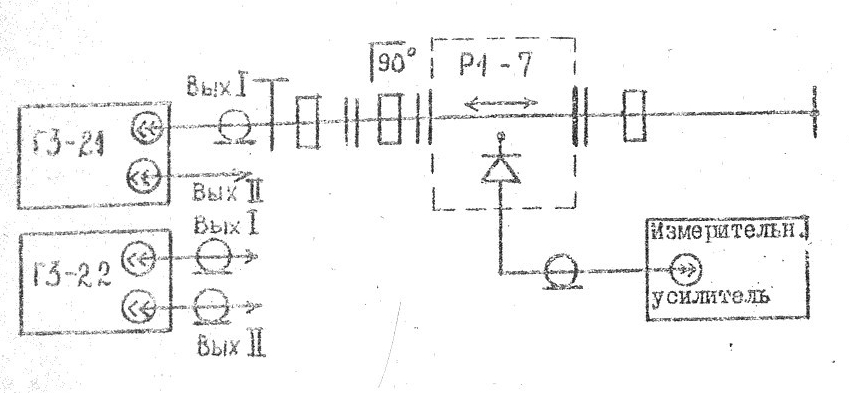
\includegraphics[width=\textwidth]{scheme.jpg}
    \end{center}
    \vspace{-20pt}
    \caption{Принципиальная схема лабораторной установки}
    \label{fig:scheme}
\end{figure}

\newpage
\section{Результаты измерений и вычислений}
\subsection{Измерения и вычисления}
\subsubsection{$\Delta\phi_{расч}$}
$$
\left.
\begin{aligned}
    \lambda_d &=\frac{\lambda}{\sqrt{1 - (\lambda/2\alpha)^2}}\\
    \phi_\tau &=\frac{2\pi}{\lambda_d}d\\
    \phi_n &= \frac{2\pi}{\lambda}d\\
    \lambda &= \frac{c}{f}\\
    \Delta\phi_{расч} &= \phi_\tau - \phi_n\\
\end{aligned}
\right\}
\Longrightarrow
\left|
\begin{aligned}
    c &= 3\cdot10^8 m/s\\
    f &= 11.96\cdot10^9Hz\\
    \alpha &= 20\cdot10^{-3}m\\
    d &= 24\cdot10^{-3}m\\
\end{aligned}
\right|
\Longrightarrow
\left|
\begin{aligned}
    \lambda &= 25\cdot10^{-3}m\\
    \lambda_d &= 32\cdot10^{-3}m\\
    \phi_\tau &= 4.71\\
    \phi_n &= 6.03\\
    \Delta\phi_{расч} &= -1.32
\end{aligned}
\right.
$$
\vspace{10 pt}
\subsubsection{$\Delta\phi_{изм}$}
Значение сдвига фаз, полученное на основе экспериментальных данных, вычисляется по формуле:
\begin{equation}
    \Delta\phi = \arctg \left[ \frac{2r}{(1+r^2)\sin^2\beta_0} \right]
\end{equation}

\vspace{10 pt}
На основе данных таблицы 3 протокола измерений (см. Приложение 1) были получены следующие значения сдвига фаз:
\begin{equation}
    \begin{aligned}
        \Psi&=15^\circ & \Delta\phi_{изм} &= 1.25\\
        \Psi&=-15^\circ & \Delta\phi_{изм} &= 1.31\\
        \vspace{5 pt}
        \Psi&=30^\circ & \Delta\phi_{изм} &= -0.95\\
        \Psi&=-30^\circ & \Delta\phi_{изм} &= -0.89\\
    \end{aligned}
\end{equation}

Хорошо видно, что значение смещения очень точно совпадает с теоретической оценкой для $\Psi=15^\circ$ 
и довольно сильно расходится при $\Psi=30^\circ$. Это может объясняться накопленной погрешностью измерительных
приборов и увеличением влияния окружающих неучтеных препятствий с увеличением угла отклонения.
\vspace{10 pt}
\subsubsection{Коэффициент эллиптичности без учета различного затухания составляющих вектора}

\begin{equation}
\lambda = \frac{\Lambda}{\sqrt{1 +
            \left( \frac{\Lambda}{2a} \right)^2}}
\end{equation}

$$
\left.
\begin{aligned}
    r_1 &= \sqrt{\frac{\alpha_{+45}}{\alpha_{-45}}}\\
    B &= \sqrt{\frac{\alpha_n}{\alpha_\tau}}\\
\end{aligned}
\right\}
\Longrightarrow
\left|
\begin{aligned}
    r_1 &= \sqrt{\frac{46}{42}} = 1.0465\\
    r_1B &= \sqrt{\frac{40}{32}}\cdot 1.0465 = 1.17\\
\end{aligned}
\right.
$$

\newpage
\subsection{Таблицы результатов измерений и вычислений}
Результаты исследования линейно поляризованной волны приведены в таблице
\ref{tab:tab1}. Полученные характеристики эллиптически поляризованных
волн сведены в эту же таблицу для компактности и удобства.
Графы таблиц, дублирующие таблицы протокола измерений (см. Приложение 1),
здесь приведены не будут.
\begin{centering}
\begin{table}[h!]
\newcolumntype{W}{D{.}{.}{2.3}}
%\begin{adjustwidth}{-1.5cm}{}
\vspace{10pt}
\begin{tabular}{cccccccccccccc} \toprule %[-2.08em]
\newcolumntype{W}{D{.}{.}{2.3}}
freq  &  z1   &  z2   &  z1'  &  z2'  &  l1    &  l2    &  L     &  lambda   &  KBv        &  lKBv     &  alpha    &  Vgroup    &  Vphase    \\
 \midrule
3000  &  1.4  &  1.7  &  8.6  &  8.3  &  1.55  &  8.45  &  13.8  &  9.92  &  0.094  &  20.44  &  59.20  &  $2.17\cdot10^8$  &  $4.14\cdot10^8$  \\
3200  &  0.5  &  2.3  &  6.6  &  8.4  &  1.4   &  7.5   &  12.2  &  9.27  &  0.609  &  4.293   &  12.44  &  $2.26\cdot10^8$  &  $3.97\cdot10^8$  \\
3600  &  2.3  &  3.3  &  7.3  &  8.4  &  2.8   &  7.85  &  10.1  &  8.24  &  0.380  &  8.382  &  24.26  &  $2.45\cdot10^8$  &  $3.67\cdot10^8$  \\
4000  &  1.5  &  1.6  &  5.8  &  5.9  &  1.55  &  5.85  &  8.6   &  7.36  &  0.042  &  27.40  &  79.34  &  $2.57\cdot10^8$  &  $3.50\cdot10^8$  \\
4200  &  1.9  &  2.0  &  6.1  &  6.2  &  1.95  &  6.15  &  8.4   &  7.24  &  0.043  &  27.25  &  78.90  &  $2.58\cdot10^8$  &  $3.48\cdot10^8$  \\
\bottomrule
\end{tabular}
\vspace{5 pt}
\caption{Исследование линейно и эллиптически поляризованных волн.} 
%\end{adjustwidth}
\label{tab:tab1}
\end{table}
\end{centering}

\subsection{Графики и рисунки}
Наиболее наглядным способом демонстрации и анализа поляризованных волн являются
поляризационные диаграммы. На рисунках \ref{fig:plot1} и \ref{fig:plot2}
представлены диаграммы для линейно и эллиптически поляризованных волн.
Они хорошо согласуются с теоретическими формами кривых, что
подтверждает корректность проведенных измерений и обработки их результатов.\\

\begin{figure}[hb!]
    \begin{center}
        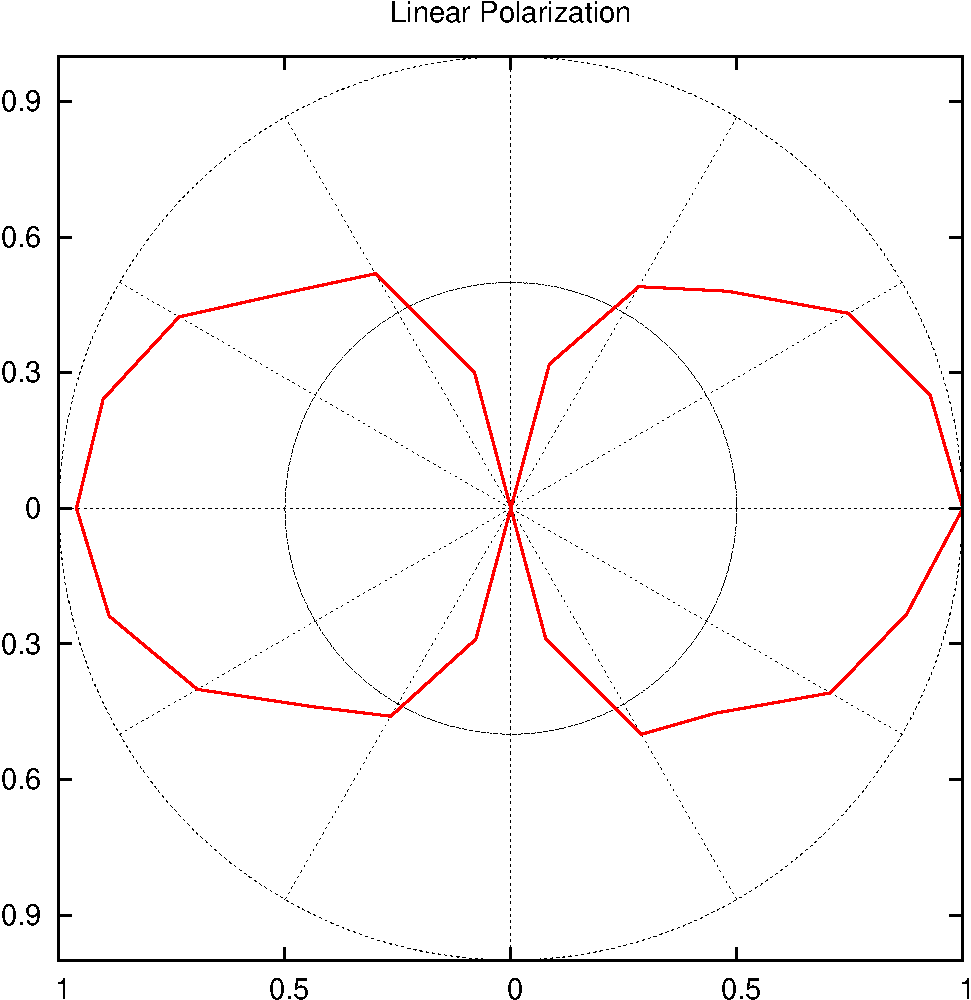
\includegraphics[width=0.65\textwidth]{data1.pdf}
    \end{center}
    \caption{Поляризационная диаграмма линейно поляризованной волны}
    \label{fig:plot1}
\end{figure}

\begin{figure}[hb!]
    \begin{center}
        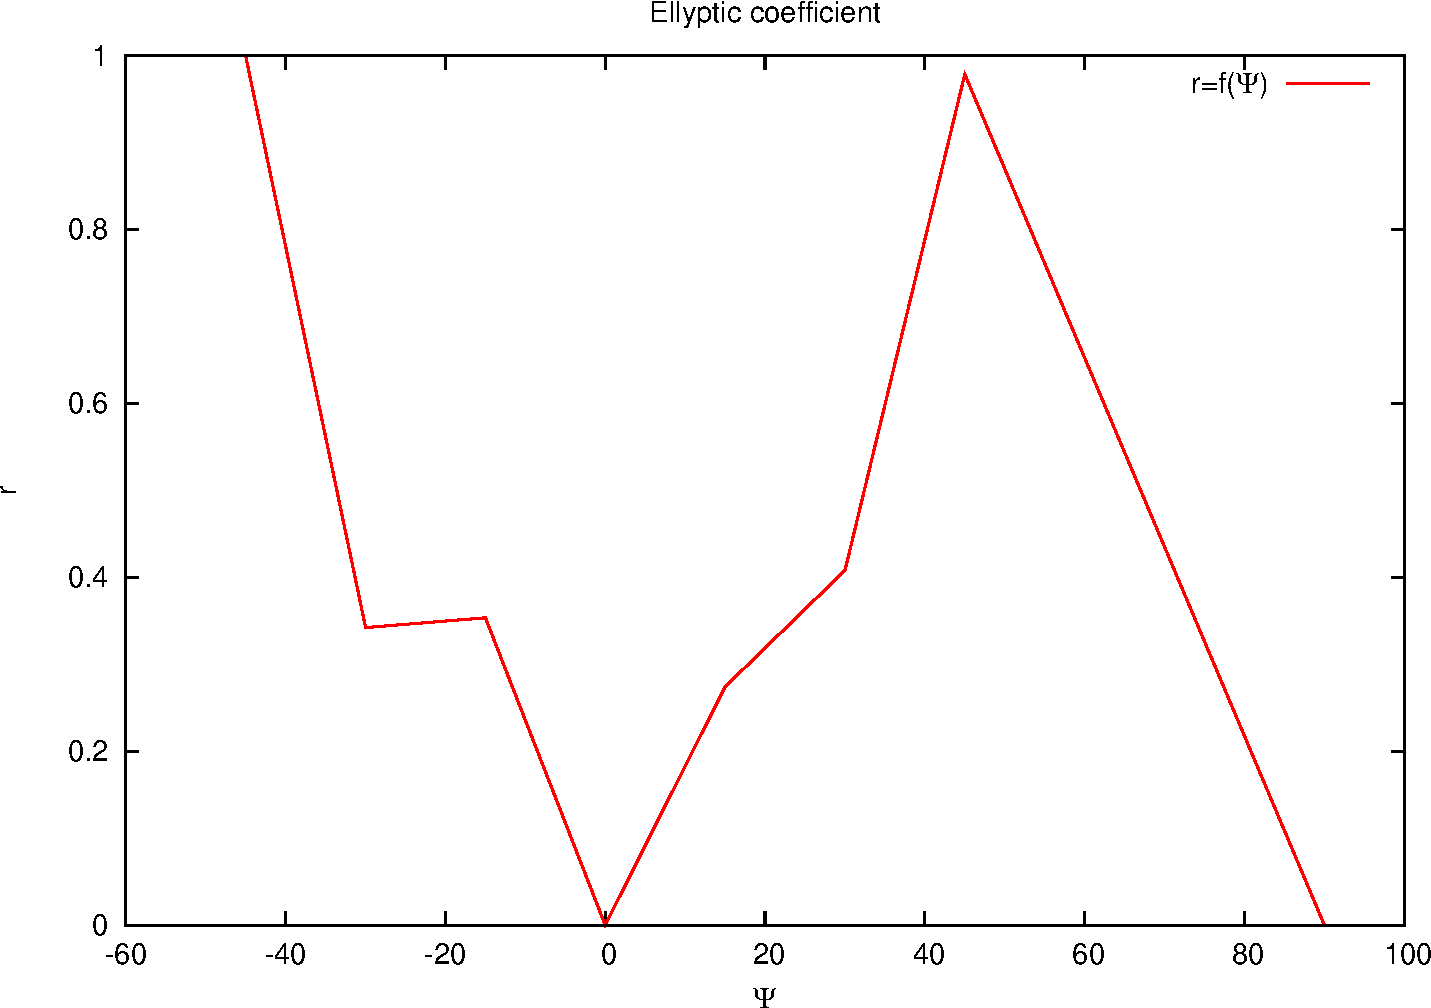
\includegraphics[width=0.89\textwidth]{data3.pdf}
    \end{center}
    \caption{График зависимости эллиптичности от угла поворота поляризационной решетки}
    \label{fig:plot3}
\end{figure}

\begin{figure}[h!]
    \begin{center}
        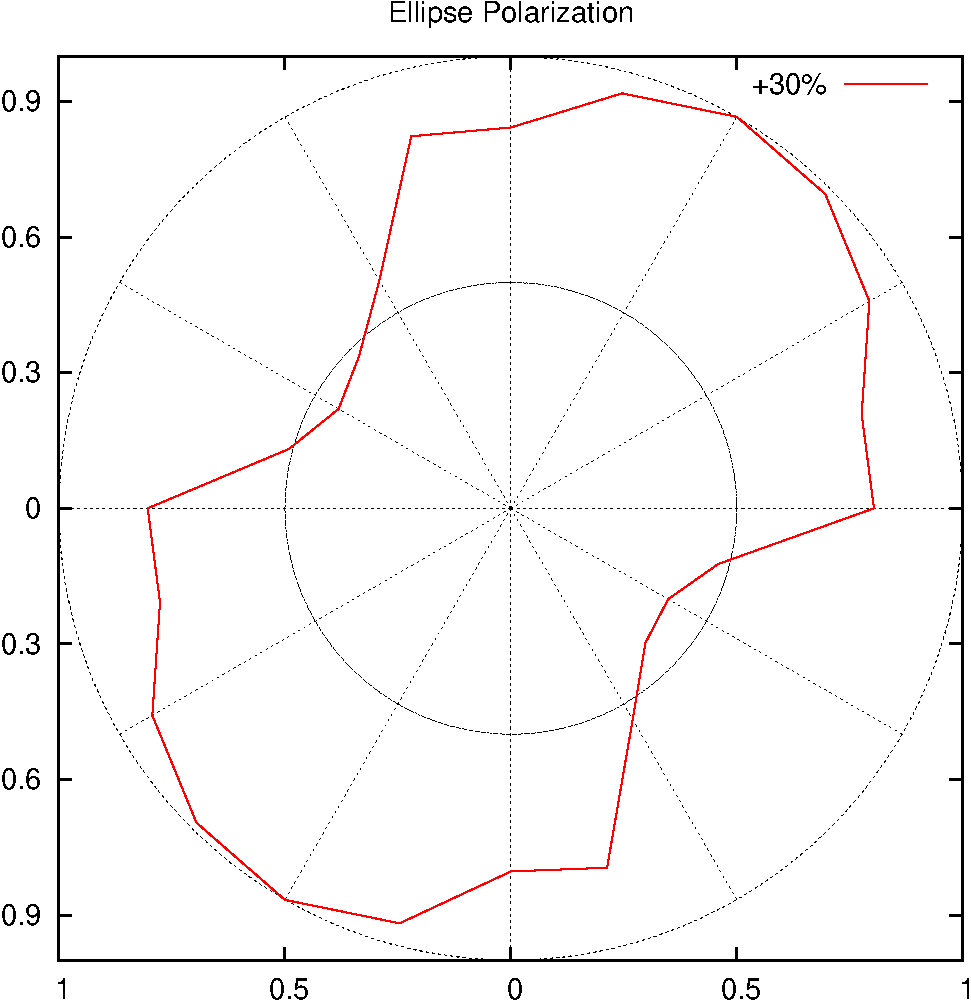
\includegraphics[width=0.7\textwidth]{data2-1.pdf}
        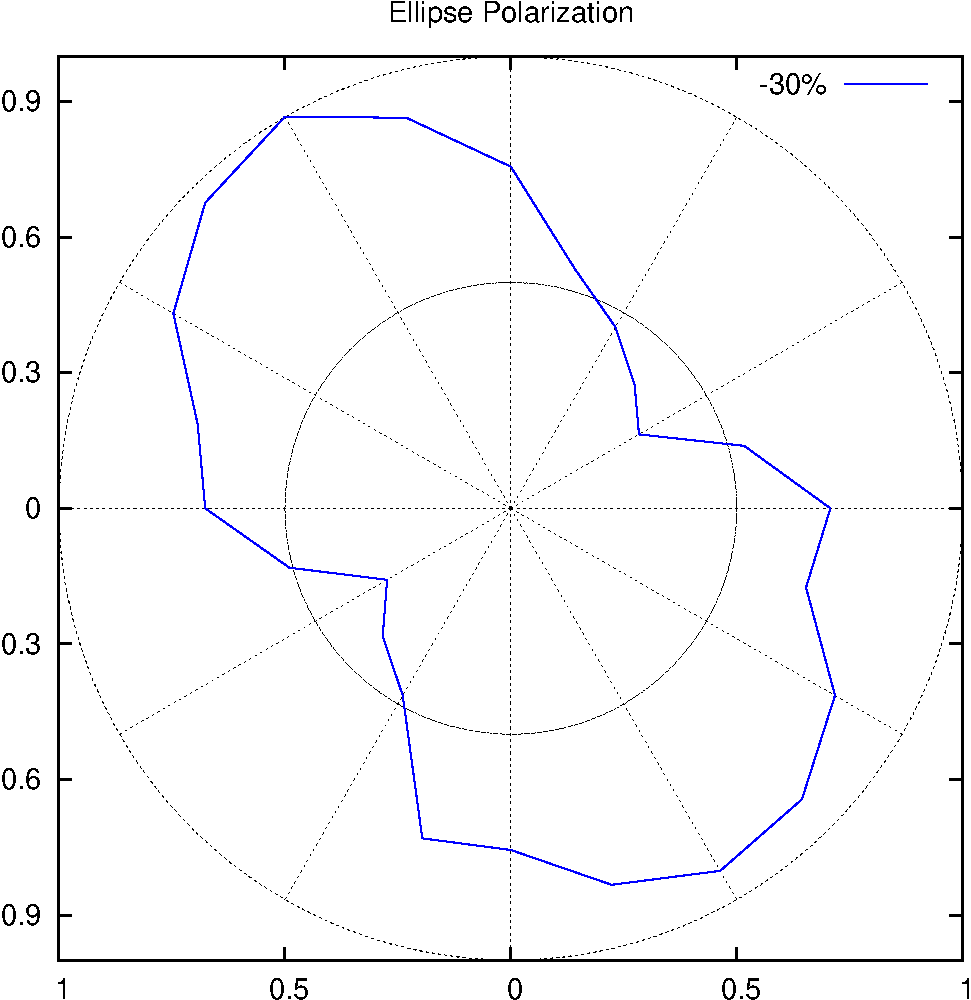
\includegraphics[width=0.7\textwidth]{data2-2.pdf}
    \end{center}
    \caption{Поляризационная диаграмма эллиптически поляризованной волны}
    \label{fig:plot2}
\end{figure}
\end{document}
